\title{Syntax and Semantics Exam}
\author{
        Benjamin Bennetzen \\
        Student ID: 20204861 \\
        Computer Science, 4th semester\\
}
\date{\today}

\documentclass[12pt]{article}

\usepackage{tikz}
\usepackage{listings}
\usepackage{mathpartir}
\usepackage{ebproof}
\usepackage{amsmath}
\usepackage[utf8]{inputenc}
\usepackage{amssymb}
\usepackage{graphicx}
\usepackage{stmaryrd}

\newcommand{\R}{\mathbb{R}}
\newcommand{\F}{\mathbb{F}}
\newcommand{\num}[1]{\mathcal{N}\llbracket #1 \rrbracket}

\begin{document}
\maketitle

\section{Exercise}
\subsection{}
Accepted words: 11, 10. Rejected words: 01, 0.

\subsection{}
$(0|1)^*1(0|1)$

\subsection{}
The states in the DFA will be comprised of the powerset of the states from the NFA. First we find the start state which will be the start state from the NFA unioned with everything that can be reached with empty ttransitions. The NFA has no empty transitions thus the start state will be $\{0\}$. Final states will be any states that contain $2$.

The start state.
\begin{center}
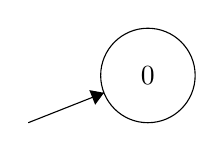
\begin{tikzpicture}[scale=0.2]
\tikzstyle{every node}+=[inner sep=0pt]
\draw [black] (20.5,-14.5) circle (3);
\draw (20.5,-14.5) node {${0}$};
\draw [black] (12.9,-17.5) -- (17.71,-15.6);
\fill [black] (17.71,-15.6) -- (16.78,-15.43) -- (17.15,-16.36);
\end{tikzpicture}
\end{center}

Add states that can be reached from the start state.
\begin{center}
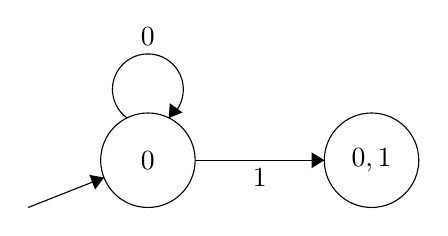
\begin{tikzpicture}[scale=0.2]
\tikzstyle{every node}+=[inner sep=0pt]
\draw [black] (20.5,-14.5) circle (3);
\draw (20.5,-14.5) node {${0}$};
\draw [black] (34.7,-14.5) circle (3);
\draw (34.7,-14.5) node {${0,1}$};
\draw [black] (12.9,-17.5) -- (17.71,-15.6);
\fill [black] (17.71,-15.6) -- (16.78,-15.43) -- (17.15,-16.36);
\draw [black] (19.177,-11.82) arc (234:-54:2.25);
\draw (20.5,-7.25) node [above] {$0$};
\fill [black] (21.82,-11.82) -- (22.7,-11.47) -- (21.89,-10.88);
\draw [black] (23.5,-14.5) -- (31.7,-14.5);
\fill [black] (31.7,-14.5) -- (30.9,-14) -- (30.9,-15);
\draw (27.6,-15) node [below] {$1$};
\end{tikzpicture}
\end{center}

Add states that can be reached from $\{0,1\}$.
\begin{center}
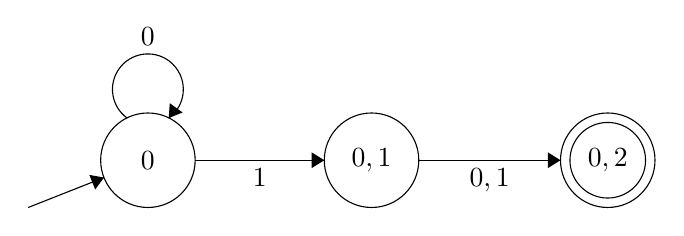
\begin{tikzpicture}[scale=0.2]
\tikzstyle{every node}+=[inner sep=0pt]
\draw [black] (20.5,-14.5) circle (3);
\draw (20.5,-14.5) node {${0}$};
\draw [black] (34.7,-14.5) circle (3);
\draw (34.7,-14.5) node {${0,1}$};
\draw [black] (49.7,-14.5) circle (3);
\draw (49.7,-14.5) node {${0,2}$};
\draw [black] (49.7,-14.5) circle (2.4);
\draw [black] (12.9,-17.5) -- (17.71,-15.6);
\fill [black] (17.71,-15.6) -- (16.78,-15.43) -- (17.15,-16.36);
\draw [black] (19.177,-11.82) arc (234:-54:2.25);
\draw (20.5,-7.25) node [above] {$0$};
\fill [black] (21.82,-11.82) -- (22.7,-11.47) -- (21.89,-10.88);
\draw [black] (23.5,-14.5) -- (31.7,-14.5);
\fill [black] (31.7,-14.5) -- (30.9,-14) -- (30.9,-15);
\draw (27.6,-15) node [below] {$1$};
\draw [black] (37.7,-14.5) -- (46.7,-14.5);
\fill [black] (46.7,-14.5) -- (45.9,-14) -- (45.9,-15);
\draw (42.2,-15) node [below] {$0,1$};
\end{tikzpicture}
\end{center}

Add states that can be reached from $\{0,2\}$.
\begin{center}
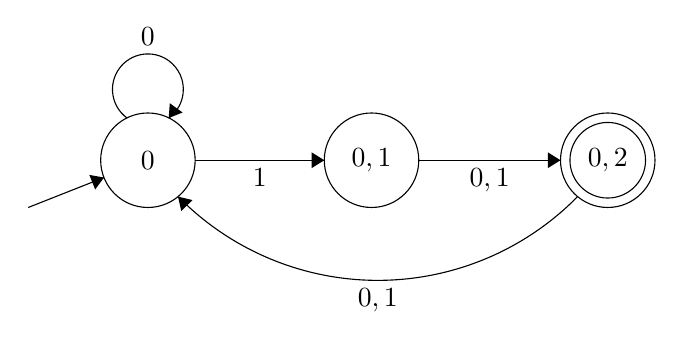
\begin{tikzpicture}[scale=0.2]
\tikzstyle{every node}+=[inner sep=0pt]
\draw [black] (20.5,-14.5) circle (3);
\draw (20.5,-14.5) node {${0}$};
\draw [black] (34.7,-14.5) circle (3);
\draw (34.7,-14.5) node {${0,1}$};
\draw [black] (49.7,-14.5) circle (3);
\draw (49.7,-14.5) node {${0,2}$};
\draw [black] (49.7,-14.5) circle (2.4);
\draw [black] (12.9,-17.5) -- (17.71,-15.6);
\fill [black] (17.71,-15.6) -- (16.78,-15.43) -- (17.15,-16.36);
\draw [black] (19.177,-11.82) arc (234:-54:2.25);
\draw (20.5,-7.25) node [above] {$0$};
\fill [black] (21.82,-11.82) -- (22.7,-11.47) -- (21.89,-10.88);
\draw [black] (23.5,-14.5) -- (31.7,-14.5);
\fill [black] (31.7,-14.5) -- (30.9,-14) -- (30.9,-15);
\draw (27.6,-15) node [below] {$1$};
\draw [black] (37.7,-14.5) -- (46.7,-14.5);
\fill [black] (46.7,-14.5) -- (45.9,-14) -- (45.9,-15);
\draw (42.2,-15) node [below] {$0,1$};
\draw [black] (47.788,-16.807) arc (-44.49305:-135.50695:17.786);
\fill [black] (22.41,-16.81) -- (22.62,-17.73) -- (23.33,-17.03);
\draw (35.1,-22.63) node [below] {$0,1$};
\end{tikzpicture}
\end{center}

\section{Exercise}
\subsection{}
\begin{lstlisting}
S -> a a A b | a B b b
A -> a A | a A b | <empty>
B -> B b | a B b | <empty>
\end{lstlisting}

\subsection{}
\begin{align*}
        S & \Rightarrow a B b b \\
          & \Rightarrow a a B b b b \\
          & \Rightarrow a a \epsilon b b b \\
\end{align*}

\begin{align*}
        S & \Rightarrow a a A b \\
          & \Rightarrow a a a A b b \\
          & \Rightarrow a a a \epsilon b b \\
\end{align*}

\subsection{}
\begin{center}
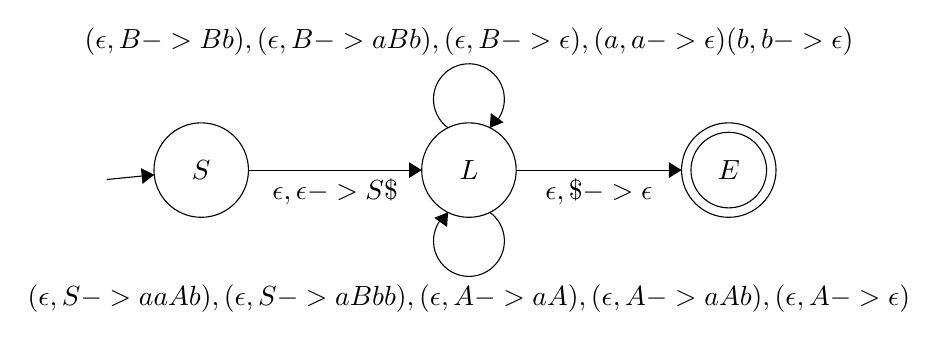
\begin{tikzpicture}[scale=0.2]
\tikzstyle{every node}+=[inner sep=0pt]
\draw [black] (19.3,-23.2) circle (3);
\draw (19.3,-23.2) node {$S$};
\draw [black] (36.3,-23.2) circle (3);
\draw (36.3,-23.2) node {$L$};
\draw [black] (52.8,-23.2) circle (3);
\draw (52.8,-23.2) node {$E$};
\draw [black] (52.8,-23.2) circle (2.4);
\draw [black] (13.3,-23.8) -- (16.31,-23.5);
\fill [black] (16.31,-23.5) -- (15.47,-23.08) -- (15.57,-24.08);
\draw [black] (22.3,-23.2) -- (33.3,-23.2);
\fill [black] (33.3,-23.2) -- (32.5,-22.7) -- (32.5,-23.7);
\draw (27.8,-23.7) node [below] {$\epsilon,\epsilon->S\$$};
\draw [black] (39.3,-23.2) -- (49.8,-23.2);
\fill [black] (49.8,-23.2) -- (49,-22.7) -- (49,-23.7);
\draw (44.55,-23.7) node [below] {$\epsilon,\$->\epsilon$};
\draw [black] (37.623,-25.88) arc (54:-234:2.25);
\draw (36.3,-30.45) node [below] {$(\epsilon,S->aaAb),(\epsilon,S->aBbb),(\epsilon,A->aA),(\epsilon,A->aAb),(\epsilon,A->\epsilon)$};
\fill [black] (34.98,-25.88) -- (34.1,-26.23) -- (34.91,-26.82);
\draw [black] (34.977,-20.52) arc (234:-54:2.25);
\draw (36.3,-15.95) node [above] {$(\epsilon,B->Bb),(\epsilon,B->aBb),(\epsilon,B->\epsilon),(a,a->\epsilon)(b,b->\epsilon)$};
\fill [black] (37.62,-20.52) -- (38.5,-20.17) -- (37.69,-19.58);
\end{tikzpicture}
\end{center}

\section{Exercise}
We assume $L'$ to be context-free, in which case there of length $p$ for which all three conditions must hold. We choose the word $a^pb^{2p}c^p \in L'$ which is clearly longer than $p$. We split this word in all possible ways and prove that $L'$ cannot be context-free.

In any given split $vxy$ will fall into any of the five instances. All $a$'s, a mix of $a$'s and $b$'s, all $b$'s, a mix of $b$'s and $c$'s.

From condition 2 we know that $v$ or $y$ will always consists of at least one character. We exploit this fact in all cases.

Case 1 $uv^0xy^0z \notin L'$ because at least one $a$ will be removed and thus there is not an equal number of $a$'s and $c$'s.

Case 2 $uv^0xy^0z \notin L'$ In this case loose any a's the argument from case 1 applies. If we only loose b's the argument from case 3 applies.

Case 3 $uv^0xy^0z \notin L'$ If we only loose b's then there be at the most an equal number of b's as there are a's and c's which will not be a word in the language.

Case 4 $uv^0xy^0z \notin L'$ If we loose any c's argument for case 5 applies. If we only loose b's argument for case 3 applies.

Case 5 $uv^0xy^0z \notin L'$ If we only loose c's then there will not be an equal amount of a's and c's which will not be a word in the language.

\section{Exercise}
\subsection{}
\begin{prooftree}
        \infer0[by rule 1]{a \rightarrow 1}
        \infer1[by rule 2]{aa \rightarrow \mid aa \mid \cdot 1}
\end{prooftree}

\subsection{}
We have the base case for $n=1$ in which case we can only use rule 1. Where we can see that $a^1 \rightarrow 1$, which holds the property.

We can then move on to the induction step $a^{n+1} = aa^n$ by the induction hypothesis we have that $a^n \rightarrow n!$. Following rule 2 we get the following. $a^{n+1} \rightarrow \mid a^{n+1} \mid \cdot n! = (n+1) \cdot n! = (n + 1)!$. This again holds the property.


\end{document}
